%!TEX root = 3_FormalAbstraction inLTLUnderUncertainty.tex

Motivated by space exploration applications we consider an autonomous rover tasked with identifying and collecting scientific samples.


\textbf{Rover model.} Without loss of generality, we consider a simple rover model as a point mass affected by stochastic disturbances on the state transitions. We assume that the position of the rover cannot be measured exactly. 
We model its dynamics as
\begin{align}
	x_{k+1}&=\begin{bmatrix}
		1&0\\
		0&1
	\end{bmatrix} x_{k} + \begin{bmatrix}
		1&0\\
		0&1
	\end{bmatrix} u_k+ w_k\\
z_k&=\begin{bmatrix}
		1&0\\
		0&1
	\end{bmatrix}x_k+v_k
\end{align}
with $w_k\sim \CA N \left(0,\begin{bmatrix}.4&-.2\\-.2&.4\end{bmatrix}\right)$ and $v_k\sim \CA N \left(0,\begin{bmatrix}1&.1\\.1&1\end{bmatrix}\right)$

A finite abstraction $M_{syst}$ of this model is constructed as outlined in the previous section by discretizing the input space $[-1,1]^2$ with nine discrete inputs, and the state space $[-10, 10]^2$ with grid points separated by $(0.76481, 0.64426)$.

\begin{figure}
	% This file was created by matplotlib2tikz v0.6.14.
\centering
\begin{tikzpicture}
\newlength\figurewidth
\newlength\figureheight
\setlength\figurewidth{\columnwidth}
\setlength\figureheight{.4\columnwidth}
\definecolor{color0}{rgb}{0.12156862745098,0.466666666666667,0.705882352941177}

\begin{axis}[scale =.8,
xlabel={$\delta$},
ylabel={$\epsilon$},
xmin=-0.01395, xmax=0.25,
ymin=0.8, ymax=1.45222764450879,
width=\figurewidth,
height=\figureheight,
% tick align=outside,
% tick pos=left,
x grid style={lightgray!92.026143790849673!black},
y grid style={lightgray!92.026143790849673!black},
axis y line=left,
axis x line=middle,
every axis x label/.style={
    at={(ticklabel* cs:1.05)}
}
]
\addplot [semithick, color0, forget plot]
table {%
0.001 1.4272384844875
0.0167368421052632 1.22339465219428
0.0324736842105263 1.16617411196529
0.0482105263157895 1.13191279574885
0.0639473684210526 1.10601589042324
0.0796842105263158 1.08400668945514
0.0954210526315789 1.06721503359466
0.111157894736842 1.05265893349788
0.126894736842105 1.04157018327801
0.142631578947368 1.02417176675944
0.158368421052632 1.01254639660019
0.174105263157895 1.00120158889137
0.189842105263158 0.991557539021032
0.205578947368421 0.982277989301703
0.221315789473684 0.97353496742902
0.237052631578947 0.965239656823681
0.252789473684211 0.960158902624749
0.268526315789474 0.951512372393061
0.284263157894737 0.927455284061691
0.3 0.935781247731614
};
\end{axis}

\end{tikzpicture}
	\caption{Trade-off between $\epsilon$ and $\delta$.  }
\end{figure}

\textbf{Environment model.} We consider exploration in a partially unknown environment. In particular, there are two potential target regions $T_1$ and $T_2$ where the probability of encountering a sample has been assessed as 0.5 and 0.6, respectively. In addition, there are two potential obstacle regions $O_1$ and $O_2$ where estimates based on satellite imagery give probabilities 0.1 and 0.3 that the rover can not traverse the obstacle safely. For both target and obstacle regions, we assume that the true nature of the region can be measured when the rover is within a certain distance of the regions. The regions are illustrated in Figs. \ref{fig:exp1} and \ref{fig:exp2}.

This environment model can be modeled as a finite-state MDP $M_{env}$. Furthermore, we model a failure probability of 0.01 at each step with an additional MDP $M_{fail}$.

\textbf{Specification.} The objective is to collect a sample while avoiding unsafe regions. To this end, we consider the specification
\begin{equation}
	\varphi = \lozenge \texttt{sample} \land \left( \lnot \texttt{fail} \; \mathcal {U} \; \texttt{sample} \right),
\end{equation}
where the atomic proposition \texttt{sample} is true if the rover is in a target region that contains a sample, and the atomic proposition \texttt{fail} is defined as being in an obstacle region that contains an obstacle, or that the system is in failure mode.

\textbf{Results.} We consider the aggregate system $M_{syst} \times M_{env} \times M_{fail}$ which is an MDP with 9 inputs and 277182 states. The specification $\varphi$ can be converted into a deterministic finite automaton. Via \eqref{eq:prob:robust_optimal} we can synthesize a control policy. Figs. \ref{fig:exp1} and \ref{fig:exp2} depict trajectories generated by the control policies, and the estimated probability that the specification can be satisfied, under two different resolutions of the unknown environment. In both experiments only $T_2$ contains a sample, and $O_1$ contains an obstacle. The difference is that in Fig. \ref{fig:exp1} also $O_2$ contains an obstacle but in Fig. \ref{fig:exp2} this region can be safely transversed.

\begin{figure}
	\footnotesize
	\setlength\figurewidth{\columnwidth} 
	\setlength\figureheight{0.6\columnwidth} 

	% This file was created by matplotlib2tikz v0.6.14.
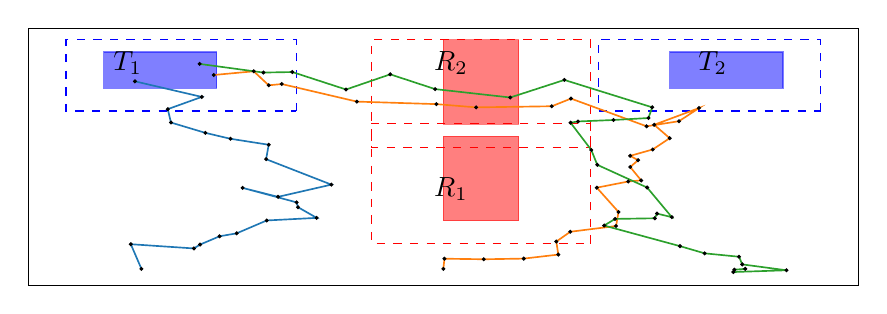
\begin{tikzpicture}

\definecolor{color1}{rgb}{1,0.498039215686275,0.0549019607843137}
\definecolor{color0}{rgb}{0.12156862745098,0.466666666666667,0.705882352941177}
\definecolor{color2}{rgb}{0.172549019607843,0.627450980392157,0.172549019607843}

\begin{axis}[
xmin=-11, xmax=11,
ymin=-10.3867095347535, ymax=10.9707956921311,
width=\figurewidth,
height=\figureheight,
mark size = 0.5,
tick align=outside,
tick pos=left,
ticks=none,
x grid style={lightgray!92.026143790849673!black},
y grid style={lightgray!92.026143790849673!black}
]
\addplot [only marks, draw=black, fill=black, colormap/viridis]
table{%
x                      y
-8.000000000000000e+00 -9.000000000000000e+00
-8.281791193811282e+00 -6.953277059756937e+00
-6.609947231673338e+00 -7.304755895777043e+00
-6.447420151999264e+00 -6.984253859219061e+00
-5.930025319876885e+00 -6.296279125763103e+00
-5.476123458484502e+00 -6.049868453584115e+00
-4.680375628377898e+00 -4.982516422756326e+00
-3.356608221836718e+00 -4.767445283086258e+00
-3.850337386959414e+00 -3.882953851781119e+00
-3.888519145722516e+00 -3.480146659512000e+00
-5.320305970691908e+00 -2.277119535242806e+00
-4.379722627893722e+00 -3.023297381626749e+00
-2.966831046751210e+00 -2.008805754832921e+00
-4.696058526749307e+00 +1.019091306738940e-01
-4.628219306657025e+00 +1.300100090541607e+00
-5.641564937919989e+00 +1.796635145522382e+00
-6.307184225641469e+00 +2.288130625455811e+00
-7.217828733789998e+00 +3.143921812081303e+00
-7.301911031188041e+00 +4.255956608402661e+00
-6.401344954223247e+00 +5.270680166902570e+00
-8.171856419883056e+00 +6.563080734161671e+00
};
\addplot [only marks, draw=black, fill=black, colormap/viridis]
table{%
x                      y
+0.000000000000000e+00 -9.000000000000000e+00
+2.985780663708154e-02 -8.155463278156050e+00
+1.071409254737555e+00 -8.202590105544974e+00
+2.130577217930679e+00 -8.147034783291767e+00
+3.046653997506764e+00 -7.814782310273142e+00
+2.993503950729483e+00 -6.732513426782055e+00
+3.364980364937721e+00 -5.919601911047740e+00
+4.577267269183741e+00 -5.442531058948178e+00
+4.641924364448064e+00 -4.277469389688367e+00
+4.066522550812239e+00 -2.261074508296681e+00
+4.900884132823335e+00 -1.747839224197386e+00
+5.242948546817821e+00 -1.658932790996332e+00
+4.951650027020791e+00 -5.458682191996806e-01
+5.160727075484096e+00 +1.786499818804538e-02
+4.951600531141017e+00 +3.796585040088483e-01
+5.548111410812660e+00 +9.093914656273503e-01
+5.998289710281388e+00 +1.845859092339660e+00
+5.586468819813884e+00 +2.958893844938534e+00
+6.773322394656686e+00 +4.341573264476058e+00
+6.244801362810041e+00 +3.255339248138960e+00
+5.386058184709245e+00 +2.832977405695359e+00
+3.382447161289477e+00 +5.131303079675625e+00
+2.874337596801116e+00 +4.495954941056568e+00
+8.693708078920757e-01 +4.402472806183647e+00
-1.833677935774903e-01 +4.671535259512195e+00
-2.290906405270350e+00 +4.881507277565658e+00
-4.280927629432187e+00 +6.338912021995005e+00
-4.626650566950111e+00 +6.233071174567763e+00
-5.024226278687982e+00 +7.396015589088654e+00
-6.083092777439494e+00 +7.089329608744675e+00
};
\addplot [only marks, draw=black, fill=black, colormap/viridis]
table{%
x                      y
+8.000000000000000e+00 -9.000000000000000e+00
+7.712479407981174e+00 -9.068560218314534e+00
+7.684857446710697e+00 -9.261842777911905e+00
+9.091886701481306e+00 -9.116022915545141e+00
+7.920264049554019e+00 -8.627351053042807e+00
+7.836372046718704e+00 -7.993013882387533e+00
+6.924714511084391e+00 -7.711316244642425e+00
+6.270580096654860e+00 -7.113203236528710e+00
+4.261157395109652e+00 -5.405610734506721e+00
+4.549567306091522e+00 -4.854291172967754e+00
+5.603414469156846e+00 -4.801669493342254e+00
+5.663344946347504e+00 -4.411676549805895e+00
+6.055644152177520e+00 -4.710990344437167e+00
+5.399991387428658e+00 -2.248963208448632e+00
+4.079080783625948e+00 -3.641899917871495e-01
+3.920155202311550e+00 +8.691698572170817e-01
+3.370749568978111e+00 +3.132663534104976e+00
+3.568671650336753e+00 +3.232289113753480e+00
+4.510831005190408e+00 +3.354928317636965e+00
+5.435609201437062e+00 +3.518835438870448e+00
+5.534818929272653e+00 +4.406944686880900e+00
+3.207427357074954e+00 +6.678357019964662e+00
+1.772408135280159e+00 +5.221828658975668e+00
-2.171849729529804e-01 +5.918511271530562e+00
-1.407705408136741e+00 +7.142892522473158e+00
-2.578687393117541e+00 +5.885635198531411e+00
-4.001703186615487e+00 +7.335332717542842e+00
-4.767609190082132e+00 +7.291363002593066e+00
-6.458371658930611e+00 +8.009045427964324e+00
};
\path [draw=red, fill=red, opacity=0.5] (axis cs:2,-5)
--(axis cs:2,2)
--(axis cs:0,2)
--(axis cs:0,-5)
--cycle;

\path [draw=red, fill=red, opacity=0.5] (axis cs:2,3)
--(axis cs:2,10)
--(axis cs:0,10)
--(axis cs:0,3)
--cycle;

\path [draw=red, fill opacity=0, dashed] (axis cs:3.9,-6.9)
--(axis cs:3.9,3.1)
--(axis cs:-1.9,3.1)
--(axis cs:-1.9,-6.9)
--cycle;

\path [draw=red, fill opacity=0, dashed] (axis cs:3.9,1.1)
--(axis cs:3.9,10)
--(axis cs:-1.9,10)
--(axis cs:-1.9,1.1)
--cycle;

\path [draw=blue, fill=blue, opacity=0.5] (axis cs:-6,6)
--(axis cs:-6,9)
--(axis cs:-9,9)
--(axis cs:-9,6)
--cycle;

\path [draw=blue, fill=blue, opacity=0.5] (axis cs:9,6)
--(axis cs:9,9)
--(axis cs:6,9)
--(axis cs:6,6)
--cycle;

\path [draw=blue, fill opacity=0, dashed] (axis cs:-3.9,4.1)
--(axis cs:-3.9,10)
--(axis cs:-10,10)
--(axis cs:-10,4.1)
--cycle;

\path [draw=blue, fill opacity=0, dashed] (axis cs:10,4.1)
--(axis cs:10,10)
--(axis cs:4.1,10)
--(axis cs:4.1,4.1)
--cycle;

\addplot [semithick, color0, forget plot]
table {%
-8 -9
-8.28179119381128 -6.95327705975694
-6.60994723167334 -7.30475589577704
-6.44742015199926 -6.98425385921906
-5.93002531987688 -6.2962791257631
-5.4761234584845 -6.04986845358412
-4.6803756283779 -4.98251642275633
-3.35660822183672 -4.76744528308626
-3.85033738695941 -3.88295385178112
-3.88851914572252 -3.480146659512
-5.32030597069191 -2.27711953524281
-4.37972262789372 -3.02329738162675
-2.96683104675121 -2.00880575483292
-4.69605852674931 0.101909130673894
-4.62821930665702 1.30010009054161
-5.64156493791999 1.79663514552238
-6.30718422564147 2.28813062545581
-7.21782873379 3.1439218120813
-7.30191103118804 4.25595660840266
-6.40134495422325 5.27068016690257
-8.17185641988306 6.56308073416167
};
\addplot [semithick, color1, forget plot]
table {%
0 -9
0.0298578066370815 -8.15546327815605
1.07140925473755 -8.20259010554497
2.13057721793068 -8.14703478329177
3.04665399750676 -7.81478231027314
2.99350395072948 -6.73251342678205
3.36498036493772 -5.91960191104774
4.57726726918374 -5.44253105894818
4.64192436444806 -4.27746938968837
4.06652255081224 -2.26107450829668
4.90088413282334 -1.74783922419739
5.24294854681782 -1.65893279099633
4.95165002702079 -0.545868219199681
5.1607270754841 0.0178649981880454
4.95160053114102 0.379658504008848
5.54811141081266 0.90939146562735
5.99828971028139 1.84585909233966
5.58646881981388 2.95889384493853
6.77332239465669 4.34157326447606
6.24480136281004 3.25533924813896
5.38605818470924 2.83297740569536
3.38244716128948 5.13130307967563
2.87433759680112 4.49595494105657
0.869370807892076 4.40247280618365
-0.18336779357749 4.6715352595122
-2.29090640527035 4.88150727756566
-4.28092762943219 6.33891202199501
-4.62665056695011 6.23307117456776
-5.02422627868798 7.39601558908865
-6.08309277743949 7.08932960874468
};
\addplot [semithick, color2, forget plot]
table {%
8 -9
7.71247940798117 -9.06856021831453
7.6848574467107 -9.26184277791191
9.09188670148131 -9.11602291554514
7.92026404955402 -8.62735105304281
7.8363720467187 -7.99301388238753
6.92471451108439 -7.71131624464243
6.27058009665486 -7.11320323652871
4.26115739510965 -5.40561073450672
4.54956730609152 -4.85429117296775
5.60341446915685 -4.80166949334225
5.6633449463475 -4.41167654980589
6.05564415217752 -4.71099034443717
5.39999138742866 -2.24896320844863
4.07908078362595 -0.36418999178715
3.92015520231155 0.869169857217082
3.37074956897811 3.13266353410498
3.56867165033675 3.23228911375348
4.51083100519041 3.35492831763697
5.43560920143706 3.51883543887045
5.53481892927265 4.4069446868809
3.20742735707495 6.67835701996466
1.77240813528016 5.22182865897567
-0.21718497295298 5.91851127153056
-1.40770540813674 7.14289252247316
-2.57868739311754 5.88563519853141
-4.00170318661549 7.33533271754284
-4.76760919008213 7.29136300259307
-6.45837165893061 8.00904542796432
};
\node at (axis cs:-0.5,-3)[
  anchor=base west,
  text=black,
  rotate=0.0
]{ $R_1$};
\node at (axis cs:-0.5,7.5)[
  anchor=base west,
  text=black,
  rotate=0.0
]{ $R_2$};
\node at (axis cs:-9,7.5)[
  anchor=base west,
  text=black,
  rotate=0.0
]{ $T_1$};
\node at (axis cs:6.5,7.5)[
  anchor=base west,
  text=black,
  rotate=0.0
]{ $T_2$};
\end{axis}

\end{tikzpicture}
	\setlength\figureheight{0.4\columnwidth} 

	% This file was created by matplotlib2tikz v0.6.14.
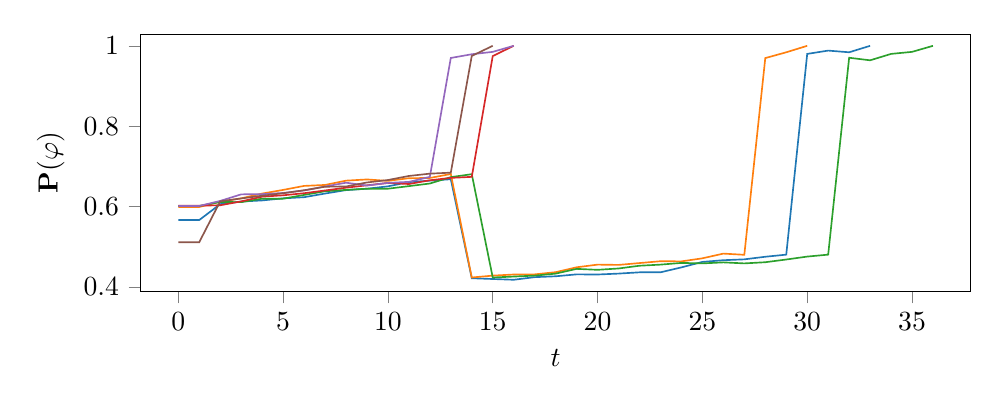
\begin{tikzpicture}

\definecolor{color1}{rgb}{1,0.498039215686275,0.0549019607843137}
\definecolor{color0}{rgb}{0.12156862745098,0.466666666666667,0.705882352941177}
\definecolor{color3}{rgb}{0.83921568627451,0.152941176470588,0.156862745098039}
\definecolor{color2}{rgb}{0.172549019607843,0.627450980392157,0.172549019607843}
\definecolor{color5}{rgb}{0.549019607843137,0.337254901960784,0.294117647058824}
\definecolor{color4}{rgb}{0.580392156862745,0.403921568627451,0.741176470588235}

\begin{axis}[
xlabel={$t$},
ylabel={$\mathbf{P}(\varphi)$},
xmin=-1.8, xmax=37.8,
ymin=0.38853456067633, ymax=1.02911740187259,
width=\figurewidth,
height=\figureheight,
tick align=outside,
tick pos=left,
x grid style={lightgray!92.026143790849673!black},
y grid style={lightgray!92.026143790849673!black}
]
\addplot [semithick, color0, forget plot]
table {%
0 0.566291945691099
1 0.566291945691099
2 0.605882976959095
3 0.612354132971019
4 0.615146535917152
5 0.620313388350838
6 0.623169341037894
7 0.632266923722546
8 0.640795190330476
9 0.64428856744584
10 0.650176429635556
11 0.660779548866506
12 0.664373678411201
13 0.667953572290617
14 0.421487160337076
15 0.419564608493884
16 0.417651962548887
17 0.424169566255033
18 0.426345484650421
19 0.431108756242508
20 0.430751120445197
21 0.433029533909929
22 0.436207218324974
23 0.436207218324974
24 0.448504360104309
25 0.462109503911388
26 0.466372172152465
27 0.468495540003818
28 0.474972821467856
29 0.480216364807438
30 0.979868029536619
31 0.988089397434187
32 0.983895865110246
33 1.00000000000003
};
\addplot [semithick, color1, forget plot]
table {%
0 0.598873106893363
1 0.598873106893363
2 0.611938797531012
3 0.620313388350838
4 0.632266923722546
5 0.641338529177884
6 0.651286575651904
7 0.653667661427169
8 0.664373678411201
9 0.667389245077004
10 0.663807726695736
11 0.670472509073791
12 0.671058796741362
13 0.680876876002895
14 0.423299602729996
15 0.428005120445258
16 0.430751120445197
17 0.431108756242508
18 0.436564779737749
19 0.448714044552832
20 0.455361601380584
21 0.454662990626655
22 0.459229983640598
23 0.463841336213989
24 0.463444874596063
25 0.471062027085172
26 0.482793941967823
27 0.479801326577619
28 0.969453775583137
29 0.983895865110246
30 1.00000000000003
};
\addplot [semithick, color2, forget plot]
table {%
0 0.601199049439663
1 0.601199049439663
2 0.611373258769312
3 0.610825977206025
4 0.61950569968835
5 0.61950569968835
6 0.628810791270583
7 0.637985226843664
8 0.641338529177884
9 0.64428856744584
10 0.64428856744584
11 0.65073129659484
12 0.657238925992285
13 0.673118973708607
14 0.680502261669169
15 0.423299602729996
16 0.425630605759241
17 0.428005120445258
18 0.432928711351226
19 0.444768945274215
20 0.442429168485533
21 0.445763301335716
22 0.452612154776499
23 0.455361601380584
24 0.459622816160484
25 0.458418097195606
26 0.460938662424354
27 0.458418097195606
28 0.461333021386082
29 0.468094526343635
30 0.475377924614331
31 0.480216364807438
32 0.970297252430312
33 0.963929119062114
34 0.979868029536619
35 0.984943443987629
36 1.00000000000003
};
\addplot [semithick, color3, forget plot]
table {%
0 0.60221316758681
1 0.60221316758681
2 0.603095656982768
3 0.612754055717539
4 0.624538495801648
5 0.62791668893401
6 0.633081343456916
7 0.639922816020793
8 0.646852485781285
9 0.652756759496805
10 0.658726606328146
11 0.655977449212481
12 0.665293062315518
13 0.671265524930602
14 0.673823637438148
15 0.974478764836217
16 1.00000000000003
};
\addplot [semithick, color4, forget plot]
table {%
0 0.601395515122941
1 0.601395515122941
2 0.61392554430982
3 0.630267741952442
4 0.630807082939585
5 0.633670305343681
6 0.639922816020793
7 0.649819559965179
8 0.659285200283324
9 0.652182261074434
10 0.658796362546444
11 0.661342844708322
12 0.673823637438148
13 0.969766480712513
14 0.979000636609888
15 0.984943431279268
16 1.00000000000003
};
\addplot [semithick, color5, forget plot]
table {%
0 0.511047337255817
1 0.511047337255817
2 0.612978700250407
3 0.620063167202848
4 0.626830204231395
5 0.633081343456916
6 0.640464676396021
7 0.649268206152165
8 0.649819559965179
9 0.659844019602223
10 0.665920200487818
11 0.67605034228333
12 0.681786379389656
13 0.684269702304902
14 0.974797775257462
15 1.00000000000003
};
\end{axis}

\end{tikzpicture}
	\caption{Above: six trajectories starting at different initial conditions. Below: estimated probability to satisfy the specification over time for the same trajectories. No sample is found in $T_1$, and $O_2$ can be safely transversed. Jumps occur in the probabilities when (non-)existence of samples are measured when the rover is close to the regions.}
	\label{fig:exp1}
\end{figure}

\begin{figure}
	\footnotesize
	\setlength\figurewidth{\columnwidth} 
	\setlength\figureheight{0.6\columnwidth} 

	% This file was created by matplotlib2tikz v0.6.14.
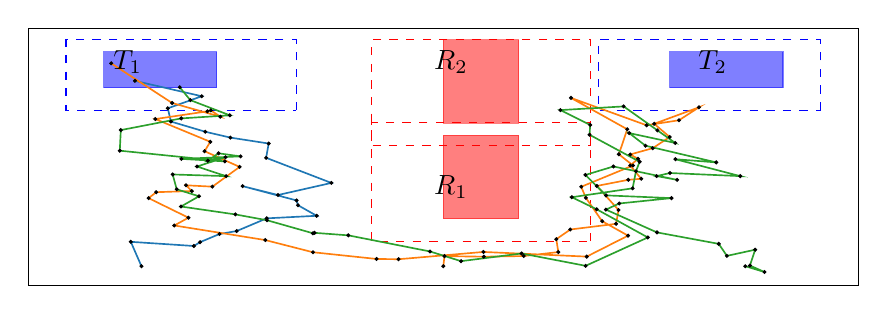
\begin{tikzpicture}

\definecolor{color1}{rgb}{1,0.498039215686275,0.0549019607843137}
\definecolor{color0}{rgb}{0.12156862745098,0.466666666666667,0.705882352941177}
\definecolor{color2}{rgb}{0.172549019607843,0.627450980392157,0.172549019607843}

\begin{axis}[
mark size = 0.5,
ticks=none,
xmin=-11, xmax=11,
ymin=-10.6290882408405, ymax=10.9823375352781,
width=\figurewidth,
height=\figureheight,
tick align=outside,
tick pos=left,
x grid style={lightgray!92.026143790849673!black},
y grid style={lightgray!92.026143790849673!black}
]
\addplot [only marks, draw=black, fill=black, colormap/viridis]
table{%
x                      y
-8.000000000000000e+00 -9.000000000000000e+00
-8.281791193811282e+00 -6.953277059756937e+00
-6.609947231673338e+00 -7.304755895777043e+00
-6.447420151999264e+00 -6.984253859219061e+00
-5.930025319876885e+00 -6.296279125763103e+00
-5.476123458484502e+00 -6.049868453584115e+00
-4.680375628377898e+00 -4.982516422756326e+00
-3.356608221836718e+00 -4.767445283086258e+00
-3.850337386959414e+00 -3.882953851781119e+00
-3.888519145722516e+00 -3.480146659512000e+00
-5.320305970691908e+00 -2.277119535242806e+00
-4.379722627893722e+00 -3.023297381626749e+00
-2.966831046751209e+00 -2.008805754832921e+00
-4.696058526749306e+00 +1.019091306738935e-01
-4.628219306657023e+00 +1.300100090541606e+00
-5.641564937919985e+00 +1.796635145522380e+00
-6.307184225641461e+00 +2.288130625455808e+00
-7.217828733789983e+00 +3.143921812081298e+00
-7.301911031188013e+00 +4.255956608402649e+00
-6.401344954223192e+00 +5.270680166902547e+00
-8.171856419882948e+00 +6.563080734161627e+00
};
\addplot [only marks, draw=black, fill=black, colormap/viridis]
table{%
x                      y
+0.000000000000000e+00 -9.000000000000000e+00
+2.985780663708160e-02 -8.155463278156050e+00
+1.071409254737555e+00 -8.202590105544974e+00
+2.130577217930679e+00 -8.147034783291767e+00
+3.046653997506764e+00 -7.814782310273142e+00
+2.993503950729483e+00 -6.732513426782055e+00
+3.364980364937721e+00 -5.919601911047740e+00
+4.577267269183741e+00 -5.442531058948178e+00
+4.641924364448064e+00 -4.277469389688367e+00
+4.066522550812240e+00 -2.261074508296681e+00
+4.900884132823337e+00 -1.747839224197387e+00
+5.242948546817824e+00 -1.658932790996334e+00
+4.951650027020797e+00 -5.458682191996835e-01
+5.160727075484108e+00 +1.786499818804027e-02
+4.951600531141041e+00 +3.796585040088380e-01
+5.548111410812709e+00 +9.093914656273301e-01
+5.998289710281483e+00 +1.845859092339620e+00
+5.586468819814069e+00 +2.958893844938457e+00
+6.773322394657046e+00 +4.341573264475908e+00
+6.244801362810740e+00 +3.255339248138667e+00
+5.386058184710604e+00 +2.832977405694789e+00
+3.382447161292124e+00 +5.131303079674516e+00
+4.874337596806267e+00 +2.495954941054408e+00
+4.650503806334480e+00 +3.995285095184848e-01
+5.025471920274055e+00 -5.406637729947061e-01
+3.653106795537211e+00 -2.331886810567701e+00
+3.777550916600270e+00 -3.262576207290882e+00
+4.208193801414156e+00 -5.223790221008551e+00
+4.894433739744199e+00 -6.435884403595750e+00
+3.799772582533073e+00 -8.195765033159091e+00
+1.063593830208735e+00 -7.803367444083015e+00
-1.186440212491861e+00 -8.416040749834128e+00
-1.769357566346293e+00 -8.393133290175719e+00
-3.454943820617372e+00 -7.829608609619289e+00
-4.718419194171268e+00 -6.806453261226547e+00
-7.128929570346833e+00 -5.582933784317277e+00
-6.754145560982441e+00 -4.927567852678047e+00
-7.809944106601641e+00 -3.287103405394836e+00
-7.608490106653687e+00 -2.786103027237490e+00
-6.664925925528791e+00 -2.687368525725410e+00
-6.819564565858922e+00 -2.207441188034236e+00
-6.119656171566637e+00 -2.321958612214557e+00
-5.398012336881704e+00 -6.633452969104143e-01
-6.326849807413460e+00 +6.558845980278348e-01
-6.175272895510815e+00 +1.444858418003883e+00
-7.632034853475458e+00 +3.355390912891568e+00
-6.251375019139898e+00 +4.004939418758159e+00
-6.160033028437569e+00 +4.084610663102694e+00
-5.910891233600980e+00 +3.553568231521559e+00
-7.187232311111987e+00 +4.703244684591716e+00
-8.802150302563509e+00 +8.035950400947264e+00
};
\addplot [only marks, draw=black, fill=black, colormap/viridis]
table{%
x                      y
+8.000000000000000e+00 -9.000000000000000e+00
+8.511205582201939e+00 -9.490847881526234e+00
+8.123691607827535e+00 -8.945490678745058e+00
+8.263822914662137e+00 -7.614276297182030e+00
+7.514100738376864e+00 -8.134440925432358e+00
+7.298345618417102e+00 -7.124767904275431e+00
+5.661620747278767e+00 -6.163981262845379e+00
+4.308129478899167e+00 -4.248895613551244e+00
+4.661943867045995e+00 -3.734081630931301e+00
+6.045638341595694e+00 -3.283722422053446e+00
+4.311200610860274e+00 -3.054620213961065e+00
+3.764155218303413e+00 -1.339286613286621e+00
+4.507407456386630e+00 -6.260285666477190e-01
+6.195941762467750e+00 -1.751868652546797e+00
+5.652298276850433e+00 -1.433432909888064e+00
+6.004475142579373e+00 -1.176455188056848e+00
+7.867024860002735e+00 -1.436677206342497e+00
+6.149524945185612e+00 -1.765396180120760e-02
+7.231136140072594e+00 -2.834317843654784e-01
+5.357245998891423e+00 +1.116871382840182e+00
+4.924762093179862e+00 +2.175740570857628e+00
+6.145247254490910e+00 +1.347818433730404e+00
+5.672732010334618e+00 +2.405018338308785e+00
+4.778200199507558e+00 +4.416354675986674e+00
+3.100685883042153e+00 +4.107914445522056e+00
+3.891391072358141e+00 +2.859356344633611e+00
+3.874517594984206e+00 +2.035479937103637e+00
+5.201506296191360e+00 -2.313046332494439e-01
+5.104339902961216e+00 -1.029190621036462e+00
+5.015533858742012e+00 -2.461605591765912e+00
+3.404566585667478e+00 -3.208436019200696e+00
+4.063604053128744e+00 -4.223179916104084e+00
+5.419276458139430e+00 -6.587904229262779e+00
+3.770997682573817e+00 -8.969356381483692e+00
+2.072826036930491e+00 -7.932486401835083e+00
+4.691549265209518e-01 -8.578316323074933e+00
-3.520651457661232e-01 -7.765184235105794e+00
-2.518265654752808e+00 -6.411080484717628e+00
-3.413207860281108e+00 -6.198922651652184e+00
-3.456088450097421e+00 -6.235552101303306e+00
-4.673123778502697e+00 -5.140669103912209e+00
-5.511881550779163e+00 -4.652643794197237e+00
-6.952415477083844e+00 -3.989299476321714e+00
-6.474737771072504e+00 -3.130571715919226e+00
-7.065234191935879e+00 -2.542851770813614e+00
-7.172383147511338e+00 -1.298336855355604e+00
-5.757402873681920e+00 -1.438398078411823e+00
-6.528591566722448e+00 -6.312978098556827e-01
-5.772384260334218e+00 +1.466319934873163e-01
-6.242081541010274e+00 -1.387082780615503e-01
-5.956475469228075e+00 +4.792766582561609e-01
-5.373508577776141e+00 +2.220560436309609e-01
-6.942001756278491e+00 +1.075019277811085e-02
-5.789985714740869e+00 -1.994507978371182e-01
-8.574179717233536e+00 +6.995122202175492e-01
-8.546440565751025e+00 +2.428342665136468e+00
-6.945052246644407e+00 +3.410292093002863e+00
-5.658246322673215e+00 +3.669916744769946e+00
-6.704820165881237e+00 +4.943999287103432e+00
-6.985289853433318e+00 +6.021483786213237e+00
};
\path [draw=red, fill=red, opacity=0.5] (axis cs:2,-5)
--(axis cs:2,2)
--(axis cs:0,2)
--(axis cs:0,-5)
--cycle;

\path [draw=red, fill=red, opacity=0.5] (axis cs:2,3)
--(axis cs:2,10)
--(axis cs:0,10)
--(axis cs:0,3)
--cycle;

\path [draw=red, fill opacity=0, dashed] (axis cs:3.9,-6.9)
--(axis cs:3.9,3.1)
--(axis cs:-1.9,3.1)
--(axis cs:-1.9,-6.9)
--cycle;

\path [draw=red, fill opacity=0, dashed] (axis cs:3.9,1.1)
--(axis cs:3.9,10)
--(axis cs:-1.9,10)
--(axis cs:-1.9,1.1)
--cycle;

\path [draw=blue, fill=blue, opacity=0.5] (axis cs:-6,6)
--(axis cs:-6,9)
--(axis cs:-9,9)
--(axis cs:-9,6)
--cycle;

\path [draw=blue, fill=blue, opacity=0.5] (axis cs:9,6)
--(axis cs:9,9)
--(axis cs:6,9)
--(axis cs:6,6)
--cycle;

\path [draw=blue, fill opacity=0, dashed] (axis cs:-3.9,4.1)
--(axis cs:-3.9,10)
--(axis cs:-10,10)
--(axis cs:-10,4.1)
--cycle;

\path [draw=blue, fill opacity=0, dashed] (axis cs:10,4.1)
--(axis cs:10,10)
--(axis cs:4.1,10)
--(axis cs:4.1,4.1)
--cycle;

\addplot [semithick, color0, forget plot]
table {%
-8 -9
-8.28179119381128 -6.95327705975694
-6.60994723167334 -7.30475589577704
-6.44742015199926 -6.98425385921906
-5.93002531987688 -6.2962791257631
-5.4761234584845 -6.04986845358412
-4.6803756283779 -4.98251642275633
-3.35660822183672 -4.76744528308626
-3.85033738695941 -3.88295385178112
-3.88851914572252 -3.480146659512
-5.32030597069191 -2.27711953524281
-4.37972262789372 -3.02329738162675
-2.96683104675121 -2.00880575483292
-4.69605852674931 0.101909130673894
-4.62821930665702 1.30010009054161
-5.64156493791999 1.79663514552238
-6.30718422564146 2.28813062545581
-7.21782873378998 3.1439218120813
-7.30191103118801 4.25595660840265
-6.40134495422319 5.27068016690255
-8.17185641988295 6.56308073416163
};
\addplot [semithick, color1, forget plot]
table {%
0 -9
0.0298578066370816 -8.15546327815605
1.07140925473755 -8.20259010554497
2.13057721793068 -8.14703478329177
3.04665399750676 -7.81478231027314
2.99350395072948 -6.73251342678205
3.36498036493772 -5.91960191104774
4.57726726918374 -5.44253105894818
4.64192436444806 -4.27746938968837
4.06652255081224 -2.26107450829668
4.90088413282334 -1.74783922419739
5.24294854681782 -1.65893279099633
4.9516500270208 -0.545868219199684
5.16072707548411 0.0178649981880403
4.95160053114104 0.379658504008838
5.54811141081271 0.90939146562733
5.99828971028148 1.84585909233962
5.58646881981407 2.95889384493846
6.77332239465705 4.34157326447591
6.24480136281074 3.25533924813867
5.3860581847106 2.83297740569479
3.38244716129212 5.13130307967452
4.87433759680627 2.49595494105441
4.65050380633448 0.399528509518485
5.02547192027405 -0.540663772994706
3.65310679553721 -2.3318868105677
3.77755091660027 -3.26257620729088
4.20819380141416 -5.22379022100855
4.8944337397442 -6.43588440359575
3.79977258253307 -8.19576503315909
1.06359383020873 -7.80336744408301
-1.18644021249186 -8.41604074983413
-1.76935756634629 -8.39313329017572
-3.45494382061737 -7.82960860961929
-4.71841919417127 -6.80645326122655
-7.12892957034683 -5.58293378431728
-6.75414556098244 -4.92756785267805
-7.80994410660164 -3.28710340539484
-7.60849010665369 -2.78610302723749
-6.66492592552879 -2.68736852572541
-6.81956456585892 -2.20744118803424
-6.11965617156664 -2.32195861221456
-5.3980123368817 -0.663345296910414
-6.32684980741346 0.655884598027835
-6.17527289551082 1.44485841800388
-7.63203485347546 3.35539091289157
-6.2513750191399 4.00493941875816
-6.16003302843757 4.08461066310269
-5.91089123360098 3.55356823152156
-7.18723231111199 4.70324468459172
-8.80215030256351 8.03595040094726
};
\addplot [semithick, color2, forget plot]
table {%
8 -9
8.51120558220194 -9.49084788152623
8.12369160782753 -8.94549067874506
8.26382291466214 -7.61427629718203
7.51410073837686 -8.13444092543236
7.2983456184171 -7.12476790427543
5.66162074727877 -6.16398126284538
4.30812947889917 -4.24889561355124
4.66194386704599 -3.7340816309313
6.04563834159569 -3.28372242205345
4.31120061086027 -3.05462021396107
3.76415521830341 -1.33928661328662
4.50740745638663 -0.626028566647719
6.19594176246775 -1.7518686525468
5.65229827685043 -1.43343290988806
6.00447514257937 -1.17645518805685
7.86702486000273 -1.4366772063425
6.14952494518561 -0.0176539618012076
7.23113614007259 -0.283431784365478
5.35724599889142 1.11687138284018
4.92476209317986 2.17574057085763
6.14524725449091 1.3478184337304
5.67273201033462 2.40501833830879
4.77820019950756 4.41635467598667
3.10068588304215 4.10791444552206
3.89139107235814 2.85935634463361
3.87451759498421 2.03547993710364
5.20150629619136 -0.231304633249444
5.10433990296122 -1.02919062103646
5.01553385874201 -2.46160559176591
3.40456658566748 -3.2084360192007
4.06360405312874 -4.22317991610408
5.41927645813943 -6.58790422926278
3.77099768257382 -8.96935638148369
2.07282603693049 -7.93248640183508
0.469154926520952 -8.57831632307493
-0.352065145766123 -7.76518423510579
-2.51826565475281 -6.41108048471763
-3.41320786028111 -6.19892265165218
-3.45608845009742 -6.23555210130331
-4.6731237785027 -5.14066910391221
-5.51188155077916 -4.65264379419724
-6.95241547708384 -3.98929947632171
-6.4747377710725 -3.13057171591923
-7.06523419193588 -2.54285177081361
-7.17238314751134 -1.2983368553556
-5.75740287368192 -1.43839807841182
-6.52859156672245 -0.631297809855683
-5.77238426033422 0.146631993487316
-6.24208154101027 -0.13870827806155
-5.95647546922808 0.479276658256161
-5.37350857777614 0.222056043630961
-6.94200175627849 0.0107501927781108
-5.78998571474087 -0.199450797837118
-8.57417971723354 0.699512220217549
-8.54644056575103 2.42834266513647
-6.94505224664441 3.41029209300286
-5.65824632267322 3.66991674476995
-6.70482016588124 4.94399928710343
-6.98528985343332 6.02148378621324
};
\node at (axis cs:-0.5,-3)[
  anchor=base west,
  text=black,
  rotate=0.0
]{ $R_1$};
\node at (axis cs:-0.5,7.5)[
  anchor=base west,
  text=black,
  rotate=0.0
]{ $R_2$};
\node at (axis cs:-9,7.5)[
  anchor=base west,
  text=black,
  rotate=0.0
]{ $T_1$};
\node at (axis cs:6.5,7.5)[
  anchor=base west,
  text=black,
  rotate=0.0
]{ $T_2$};

\end{axis}

\end{tikzpicture}

	\setlength\figureheight{0.4\columnwidth} 

	% This file was created by matplotlib2tikz v0.6.14.
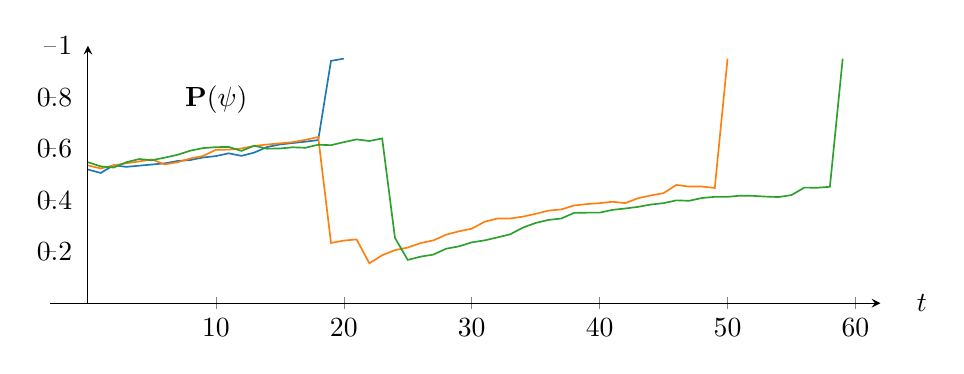
\begin{tikzpicture}

\definecolor{color1}{rgb}{1,0.498039215686275,0.0549019607843137}
\definecolor{color0}{rgb}{0.12156862745098,0.466666666666667,0.705882352941177}
\definecolor{color2}{rgb}{0.172549019607843,0.627450980392157,0.172549019607843}

\begin{axis}[
xlabel={$t$},
ylabel={$\mathbf{P}(\psi)$},
xmin=-2.95, xmax=61.95,
ymin=0.115383927583069, ymax=0.98995146727863,
width=\figurewidth,
height=\figureheight,
tick align=outside,
tick pos=left,
x grid style={lightgray!92.026143790849673!black},
y grid style={lightgray!92.026143790849673!black},
axis y line=middle,
axis x line=middle,
ymin = 0,
ymax = 1,
every axis x label/.style={
    at={(ticklabel* cs:1.05)}
},
every axis y label/.style={
    at={(0.2,0.7)},
    anchor=south,
}
]
\addplot [semithick, color0, forget plot]
table {%
0 0.519437323294361
1 0.505905967792163
2 0.535762794709806
3 0.529641473005327
4 0.534202921709494
5 0.538759248959358
6 0.543315961968619
7 0.552430637025909
8 0.556136049552841
9 0.566110510314734
10 0.571484104700144
11 0.582252336732076
12 0.572331976818973
13 0.585099080576503
14 0.606729657381389
15 0.616691491600847
16 0.622103745520534
17 0.627514467660256
18 0.63366955987662
19 0.941425688953114
20 0.950198397292469
};
\addplot [semithick, color1, forget plot]
table {%
0 0.535132433990641
1 0.52361711183953
2 0.535132433990641
3 0.543731008001737
4 0.550703063551738
5 0.558585302195194
6 0.539173994232859
7 0.547458159763064
8 0.562091024973306
9 0.572039360069865
10 0.596097657367583
11 0.596563953011597
12 0.601126871317435
13 0.611092694091856
14 0.616488991909715
15 0.621058196593617
16 0.625615820087544
17 0.634735491594122
18 0.645561482408208
19 0.234045441759929
20 0.243149052412218
21 0.247728706925773
22 0.155136997569231
23 0.186216159094014
24 0.206143993143537
25 0.21610603533654
26 0.233451571592582
27 0.244022547027297
28 0.26598938278977
29 0.279350961751404
30 0.289174863802017
31 0.316179113764902
32 0.328982444064366
33 0.328982444064366
34 0.336315254852049
35 0.347152718032949
36 0.359673571635938
37 0.364229419086882
38 0.379600870657791
39 0.38500440205473
40 0.388712554616358
41 0.394120578102893
42 0.388712554616358
43 0.407787653050549
44 0.418603916546378
45 0.427715165844223
46 0.459361669473757
47 0.453045606826443
48 0.453045606826443
49 0.44763200589673
50 0.950198397288434
};
\addplot [semithick, color2, forget plot]
table {%
0 0.547722366299717
1 0.531583463211636
2 0.527071760546219
3 0.547722366299717
4 0.560103204844214
5 0.555328267951691
6 0.565540804425142
7 0.576360127473417
8 0.592582903342865
9 0.602542902132007
10 0.606253832137332
11 0.60710633658241
12 0.591576171090529
13 0.611824096954832
14 0.600274259142499
15 0.601126871317435
16 0.605680578715834
17 0.603975733220287
18 0.615647313283849
19 0.613942290635706
20 0.625615820087544
21 0.636351488414114
22 0.630168418209078
23 0.640134983716998
24 0.253945007517459
25 0.168083558274324
26 0.180794947372842
27 0.188822613176964
28 0.211591710630682
29 0.220721176339468
30 0.236209066973026
31 0.244022547027297
32 0.255461135796253
33 0.267559897089635
34 0.293610800263249
35 0.311769872918488
36 0.323468852817987
37 0.328941635241611
38 0.350849395838469
39 0.351708421550836
40 0.351708421550836
41 0.362524629192895
42 0.367932683007021
43 0.374193140341984
44 0.383304454416872
45 0.388712554616358
46 0.399528017149535
47 0.397823889661972
48 0.408640059633355
49 0.413195587429733
50 0.413195587429733
51 0.417751484126762
52 0.416899076992805
53 0.414048005317165
54 0.412343194766756
55 0.420173604424889
56 0.449079203299998
57 0.448481084716646
58 0.452180689640779
59 0.950198397288434
};
\end{axis}

\end{tikzpicture}
	\caption{Same as Fig. \ref{fig:exp1} with the difference that both $O_1$ and $O_2$ contain obstacles.}
	\label{fig:exp2}
\end{figure}